\documentclass[a4paper]{article}
\linespread{1.6}
\usepackage{geometry}
\usepackage{setspace}
\usepackage{amsmath}
\usepackage{amssymb}
\usepackage{enumerate}
\usepackage[pdftex]{graphicx}
\usepackage{float}
\usepackage{subfigure}
\usepackage{listings}
\geometry{left=1.5cm,right=1.5cm,top=2.5cm,bottom=2.5cm}

\begin{document}
\begin{spacing}{2.0}
\begin{flushleft}\begin{huge}EEE5502 Foundations of Digital Signal Processing   Code 2\end{huge}\end{flushleft}
\begin{flushright}\begin{Large} Hudanyun Sheng \end{Large}\end{flushright}

\Large\textbf{ Question \#3}:  \\
\normalsize
\begin{enumerate}[(a)]
\item The plot of signal z is shown below:
\begin{figure} [H]
\centering
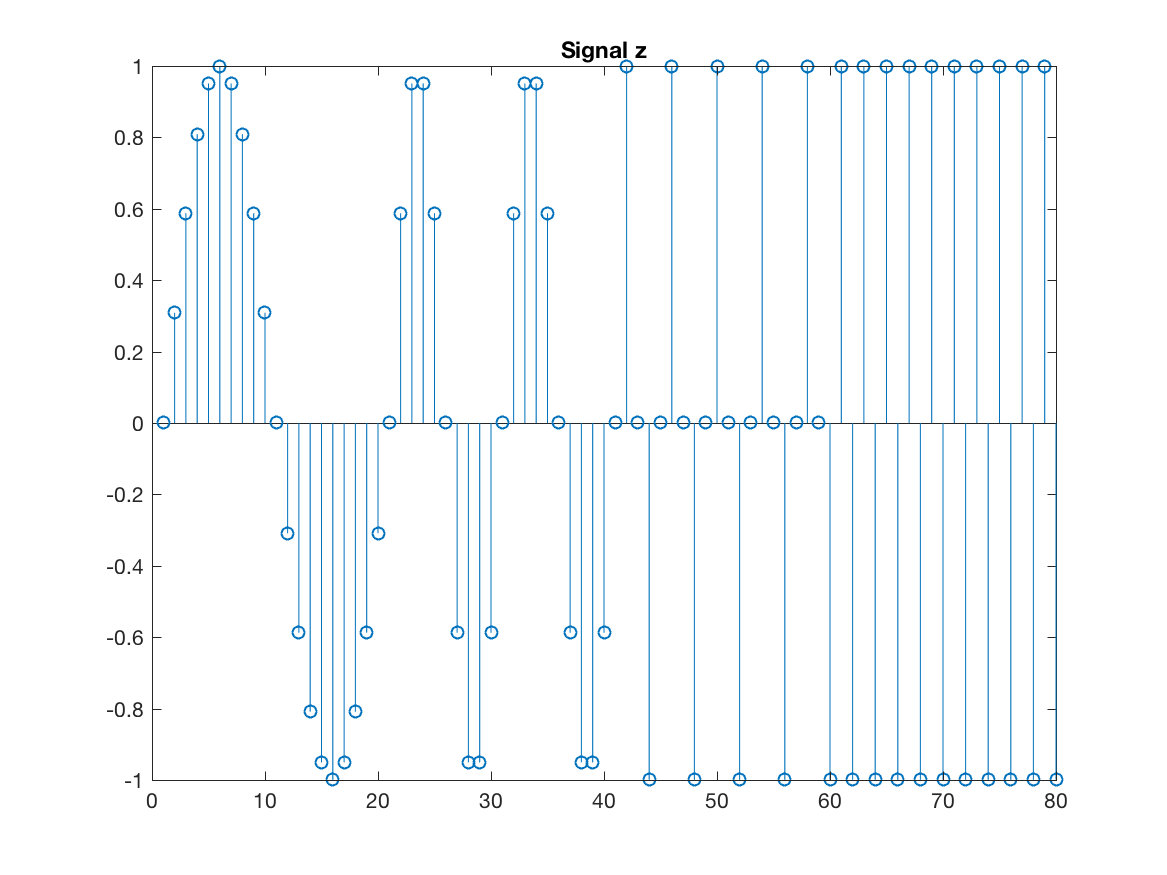
\includegraphics[width=4in,height=4in]{signalz.png}
\caption{z signal}
\label{fig:graph}
\end{figure}

\item Show below are the plots of signals y1, y2, y3, respectively:
\begin{figure} [H]
\centering
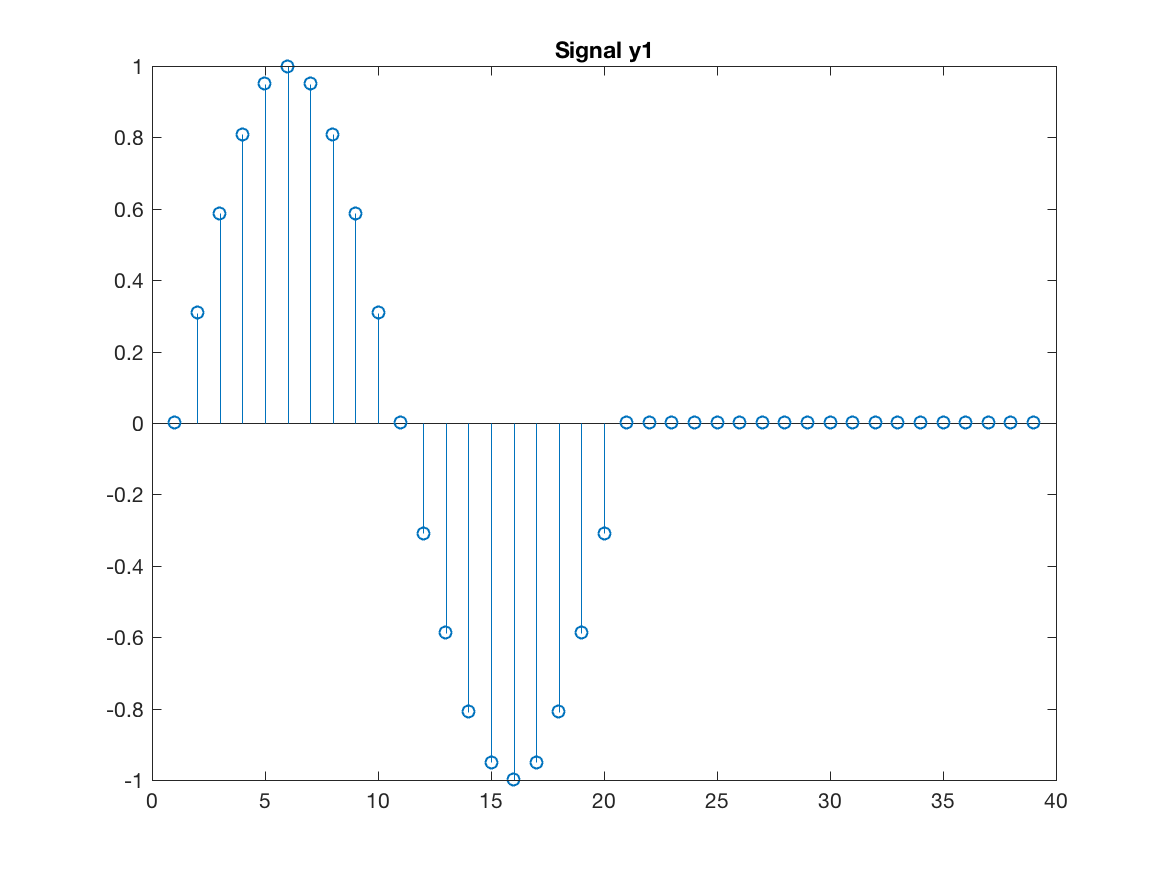
\includegraphics[width=2in,height=2in]{signaly1.png}
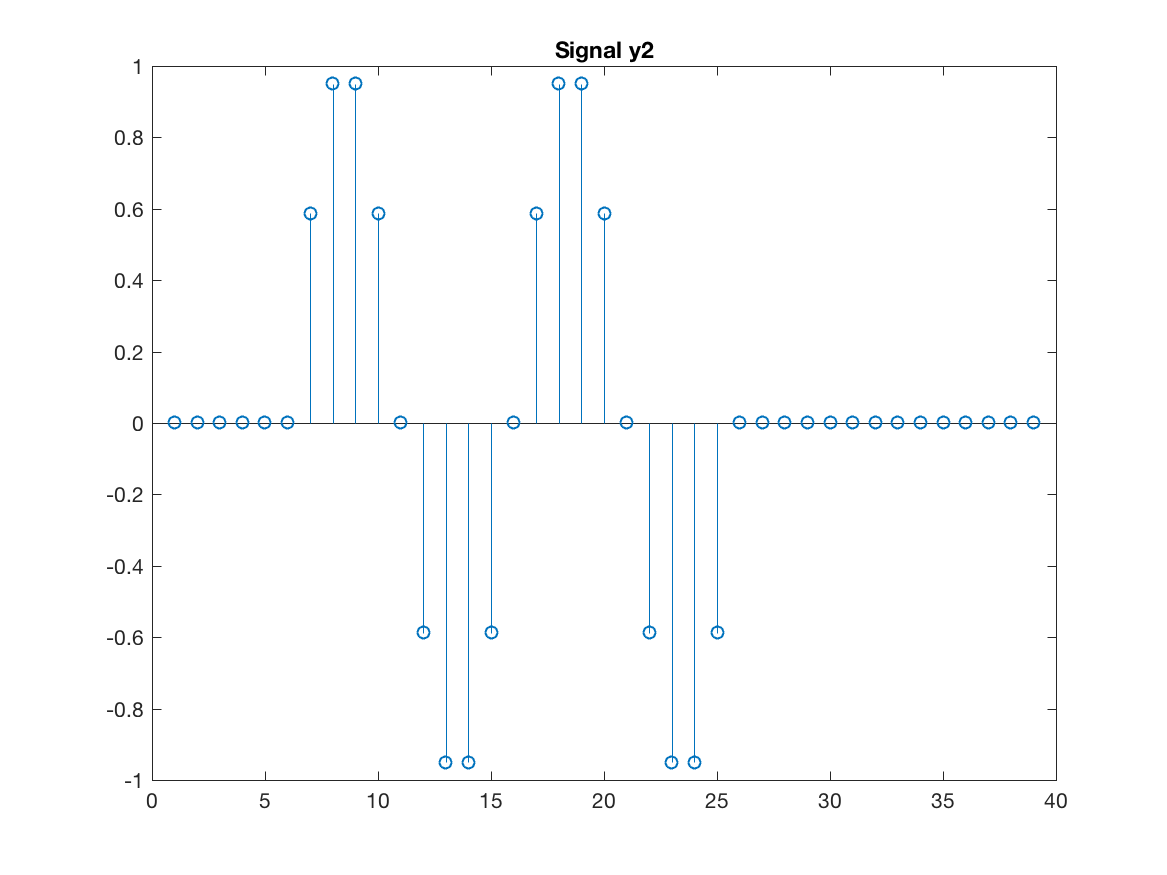
\includegraphics[width=2in,height=2in]{signaly2.png}
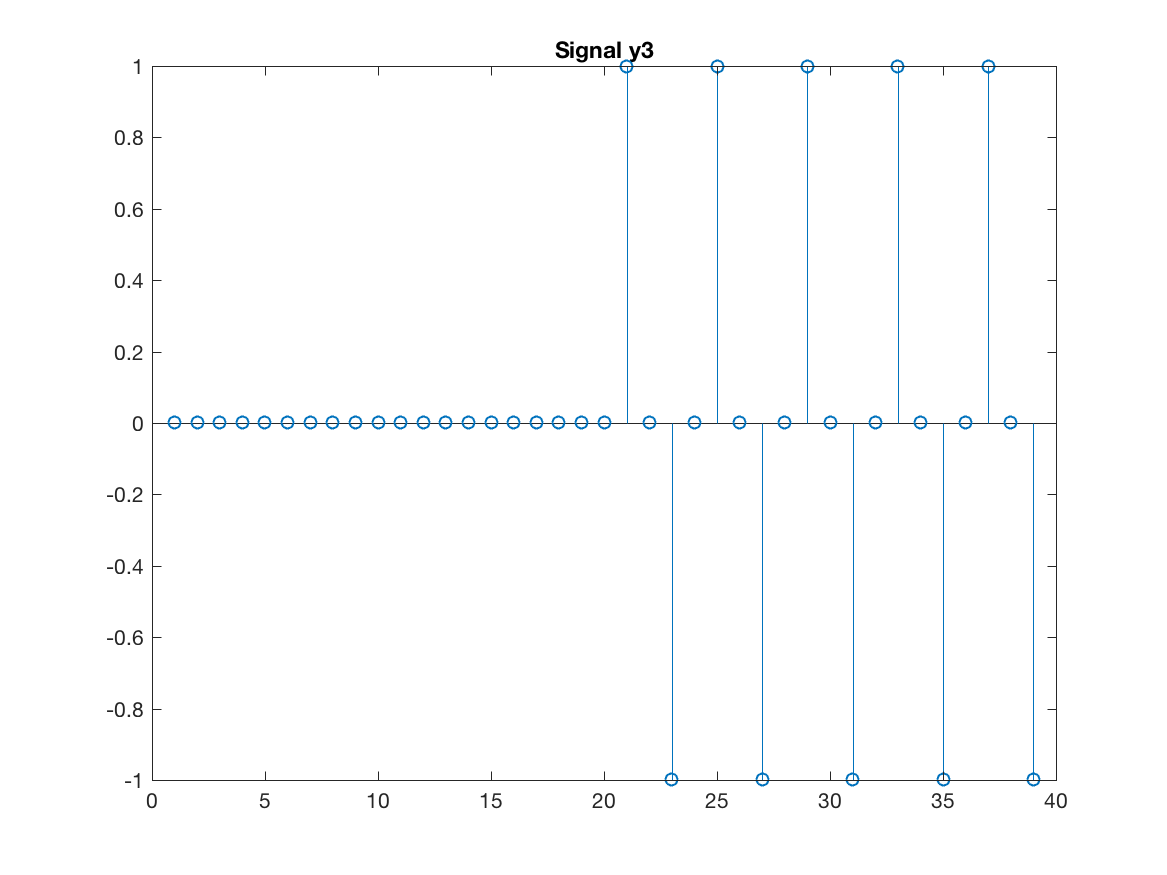
\includegraphics[width=2in,height=2in]{signaly3.png}
\caption{Signals y1, y2, y3}
\label{fig:graph}
\end{figure}

\item As discussed in the previous part (question \#2), we can see that after convolve a causal signal with length $N_x$ with another causal signal with length $N_y$, the resulting signal would have a signal with length $N_x+N_y-1$.

\end{enumerate}

\newpage
\Large\textbf{ Question \#4}:  \\
\normalsize
\begin{enumerate}[(a)]
\item The plot of auto-correlation of signal x1 with itself is shown below:
\begin{figure}[H]
\centering
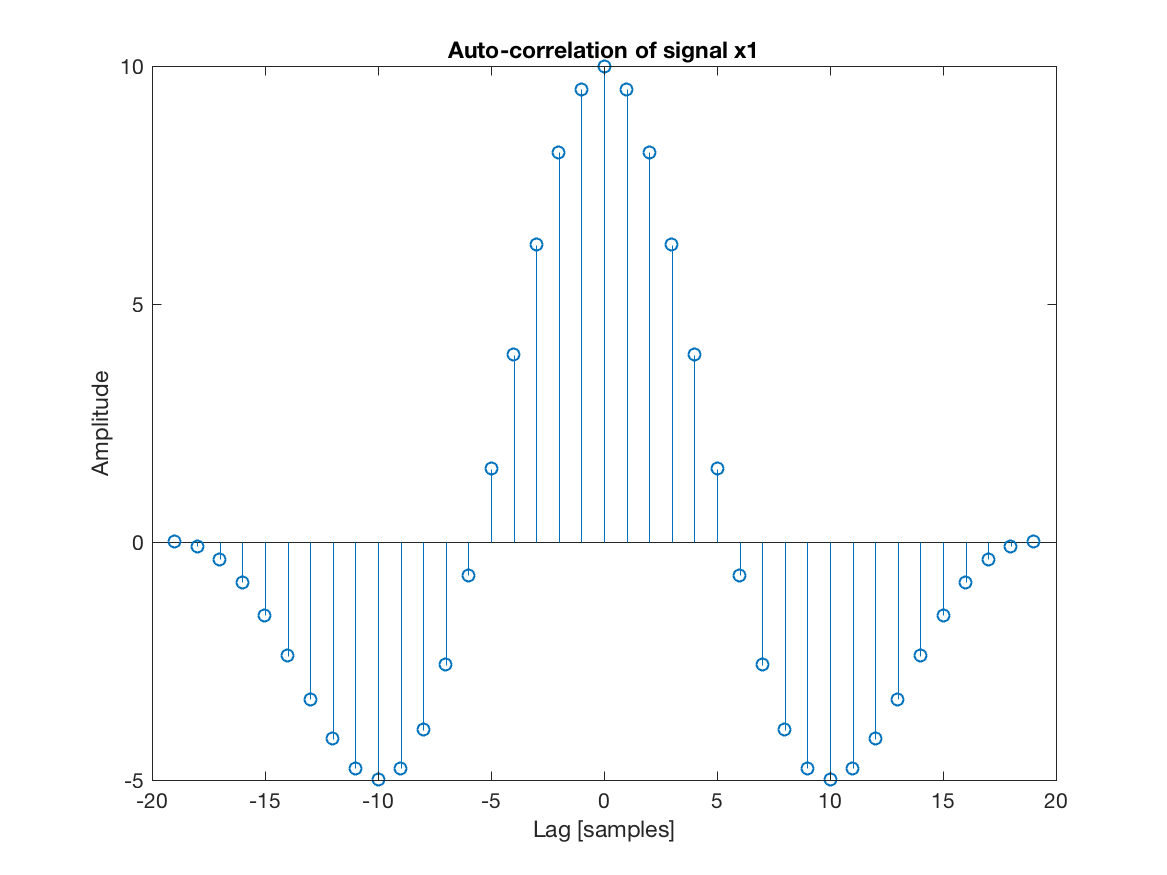
\includegraphics[width=2in,height=2in]{autox1.png}
\caption{Auto-correlation of signal x1}
\label{fig:graph}
\end{figure}

\item The plots of auto-correlation of signals x2, x3, x4 with themselves are shown below:
\begin{figure}[H]
\centering
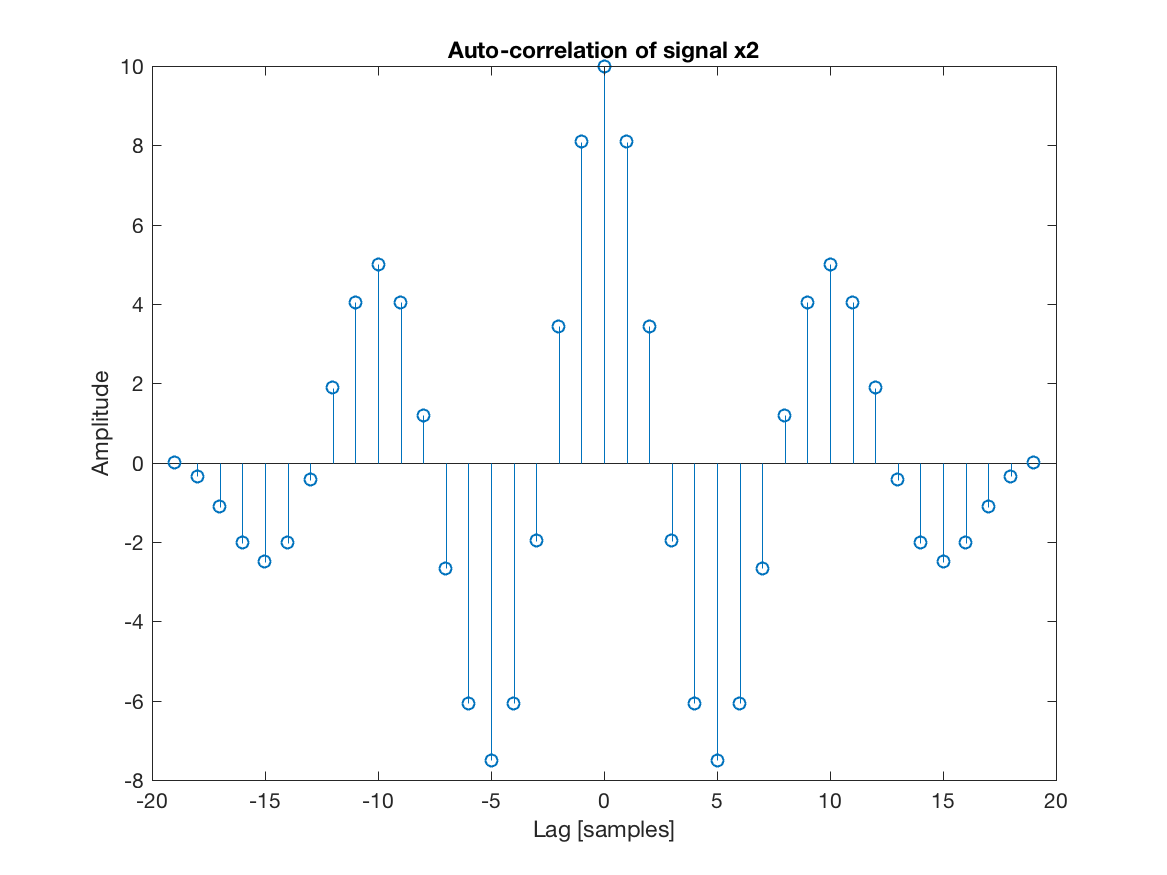
\includegraphics[width=2in,height=2in]{autox2.png}
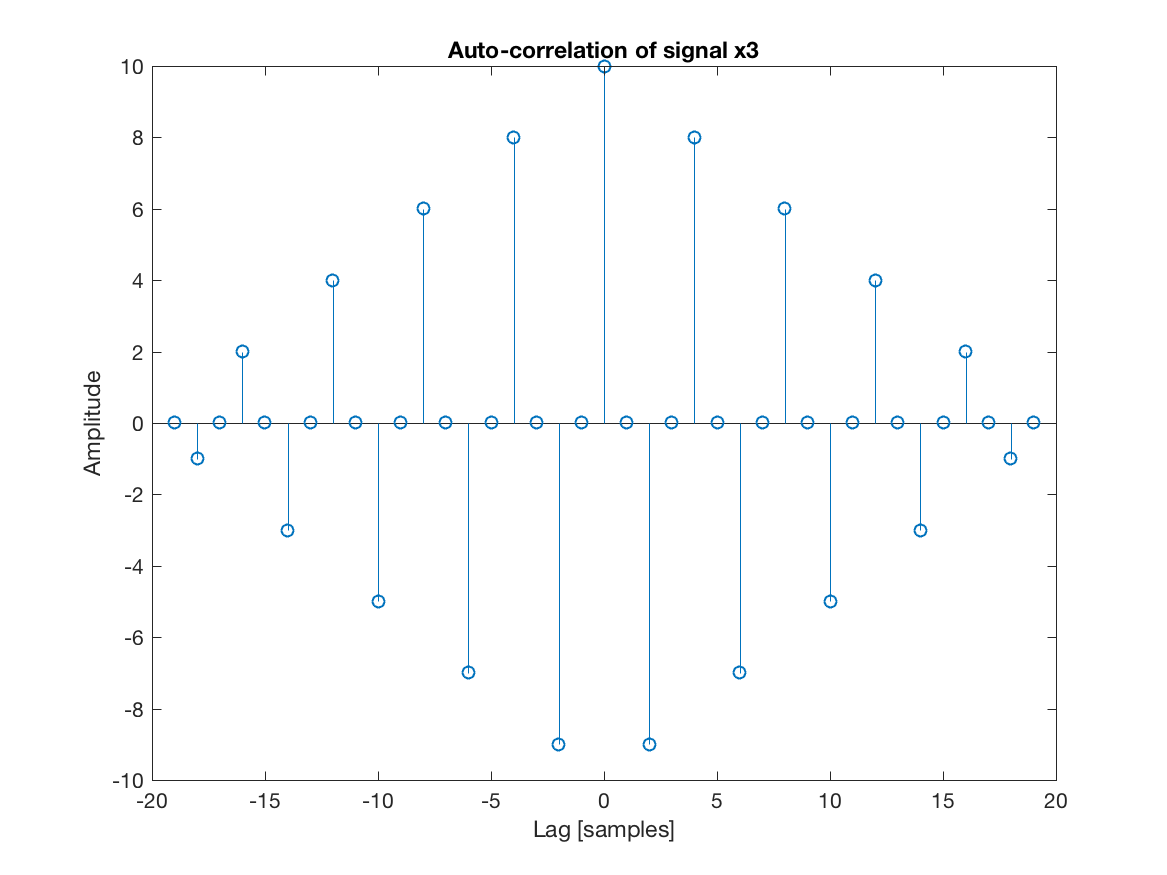
\includegraphics[width=2in,height=2in]{autox3.png}
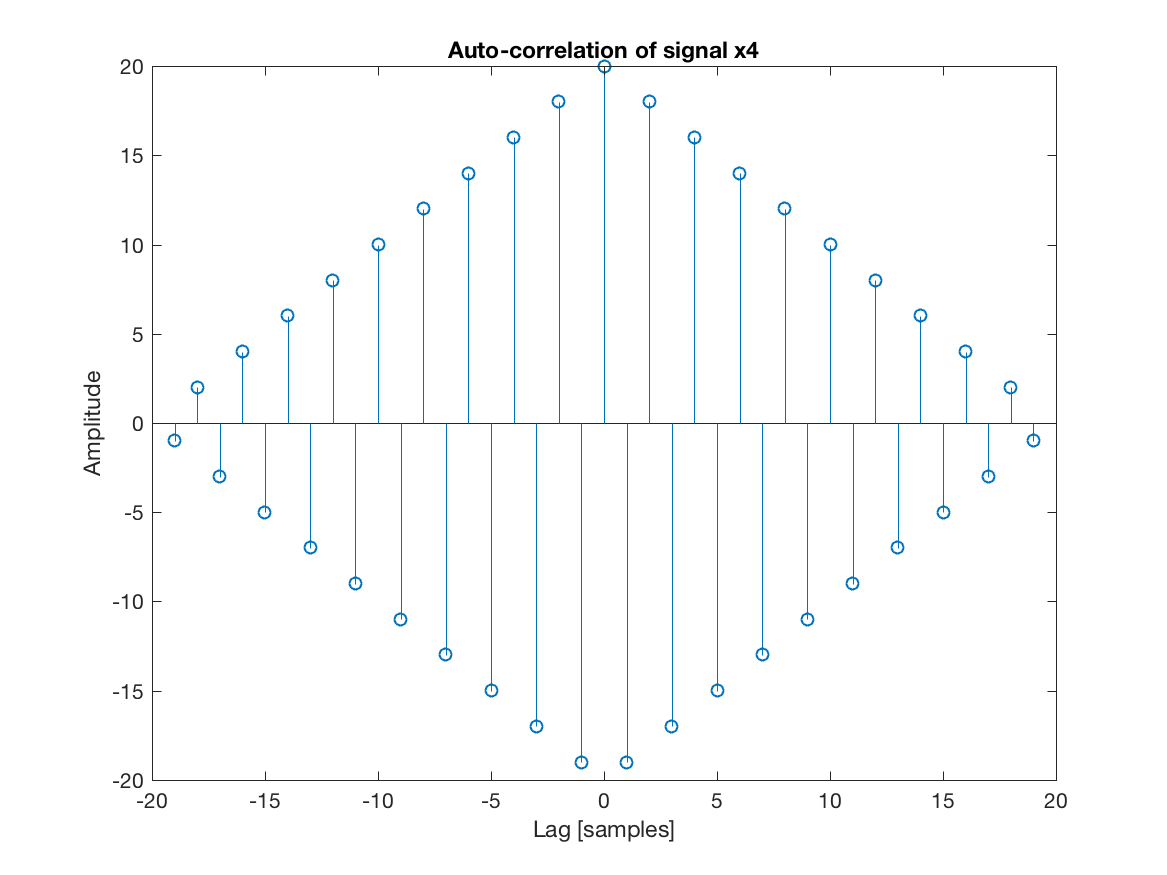
\includegraphics[width=2in,height=2in]{autox4.png}
\caption{Auto-correlations of signals x2, x3, x4}
\label{fig:graph}
\end{figure}

\item The plots of correlations between $z[n]$ and $x_1[n]$; $z[n]$ and $x_2[n]$; $z[n]$ and $x_3[n]$; $z[n]$ and $x_4[n]$ are shown below:

\begin{figure}[H]
\centering
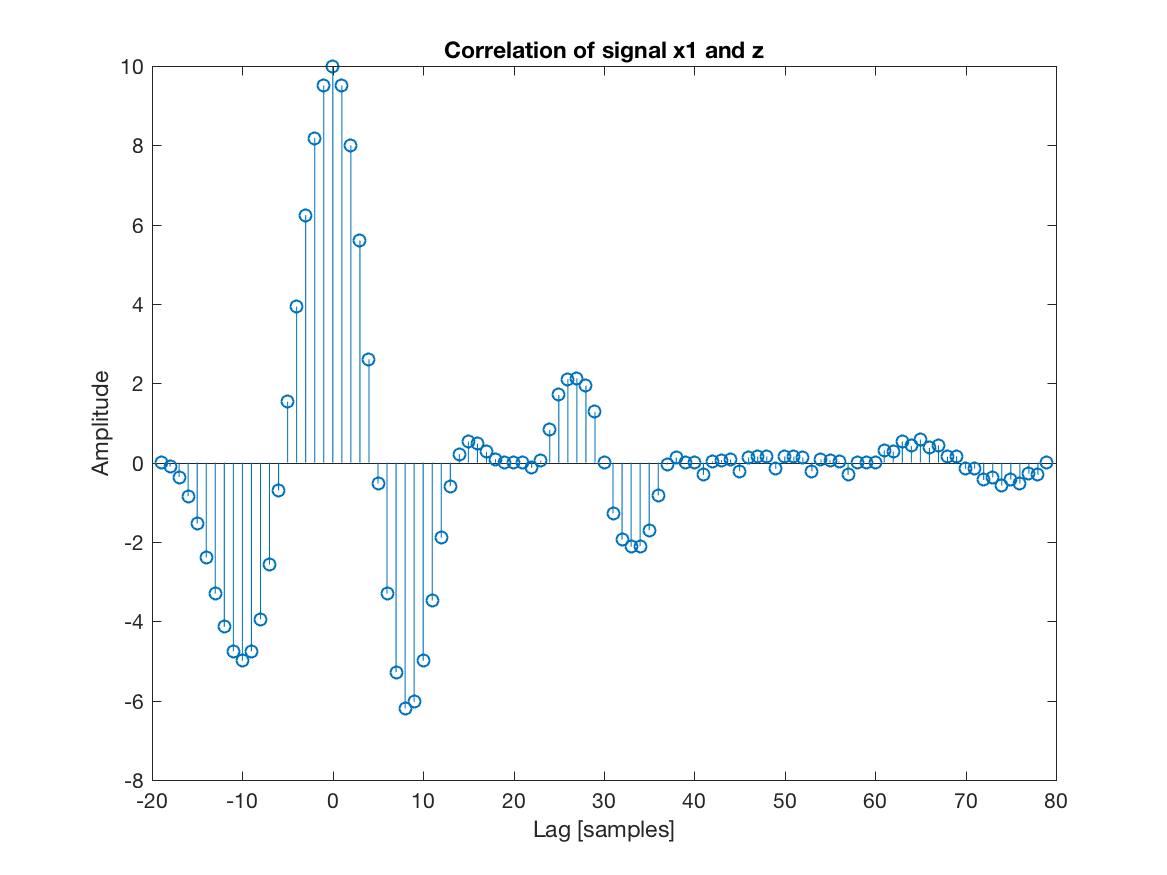
\includegraphics[width=1.7in,height=1.7in]{crossx1.png}
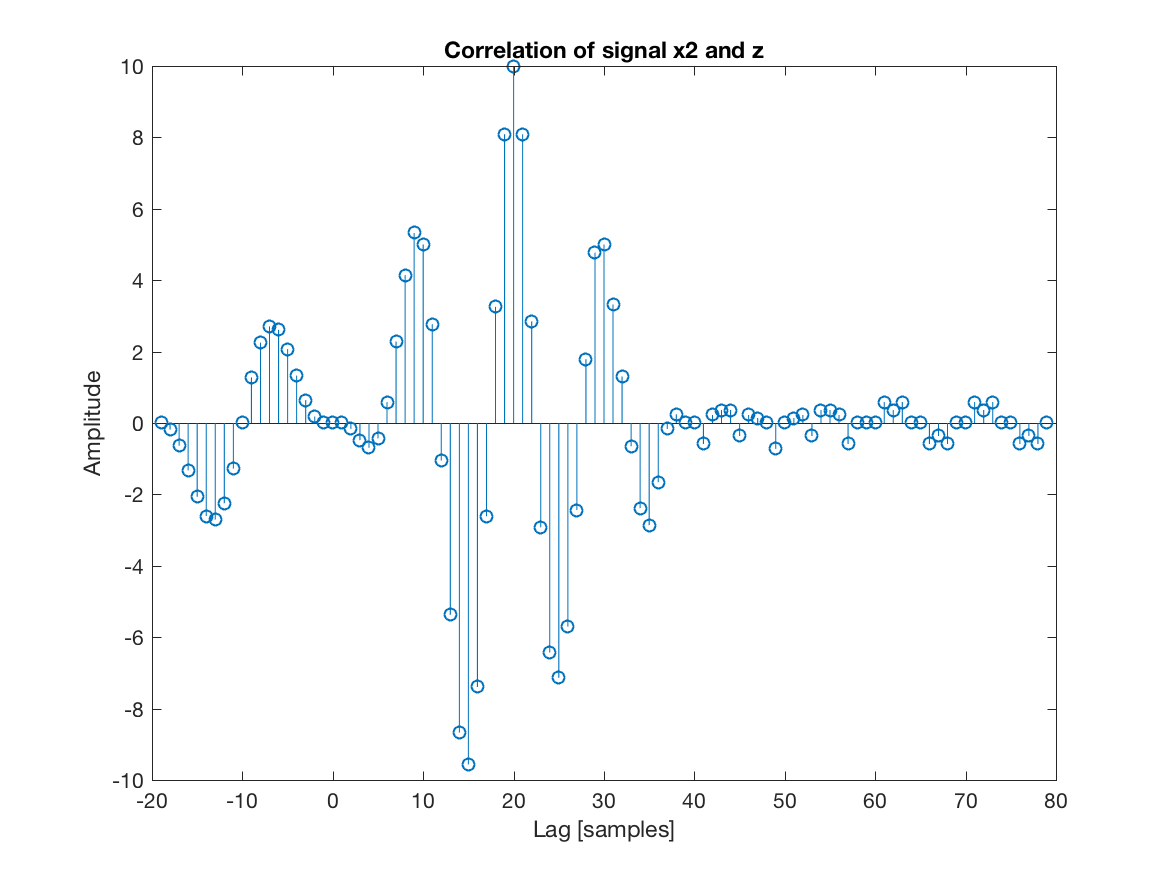
\includegraphics[width=1.7in,height=1.7in]{crossx2.png}
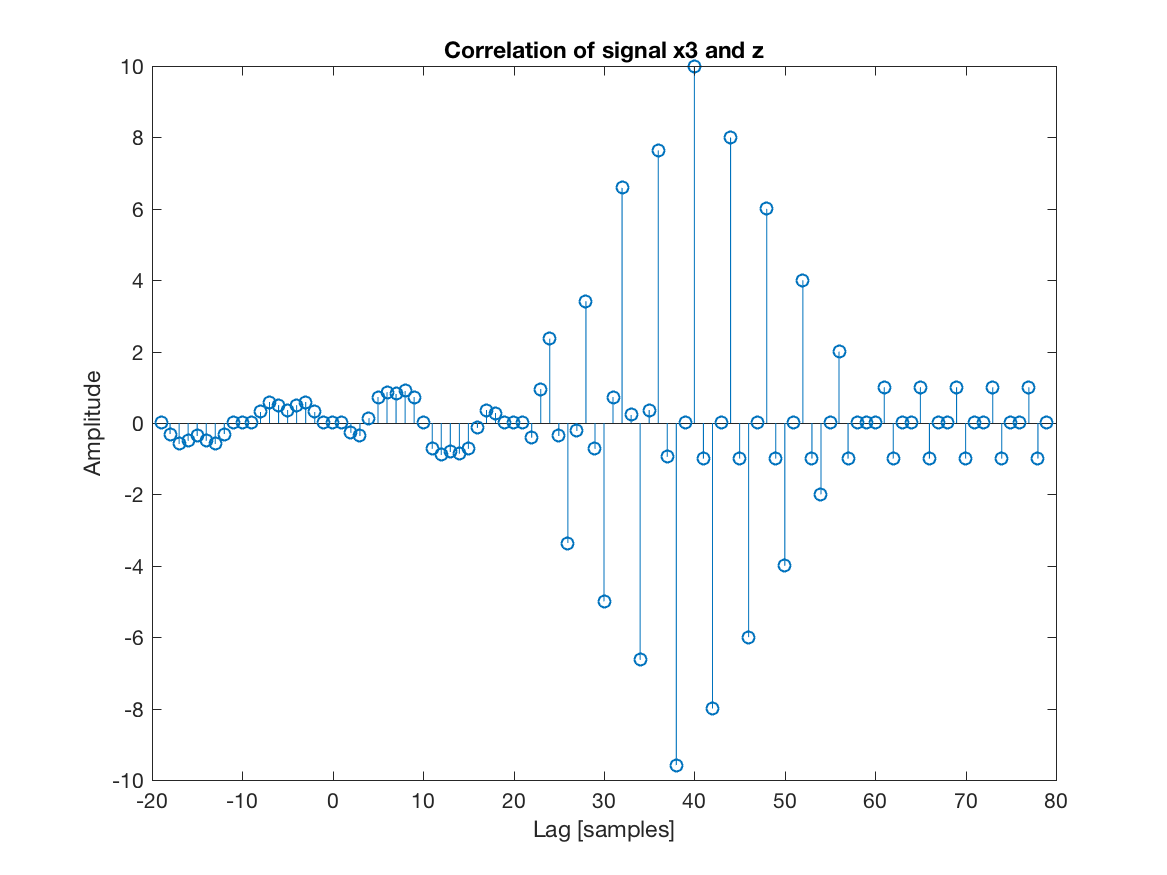
\includegraphics[width=1.7in,height=1.7in]{crossx3.png}
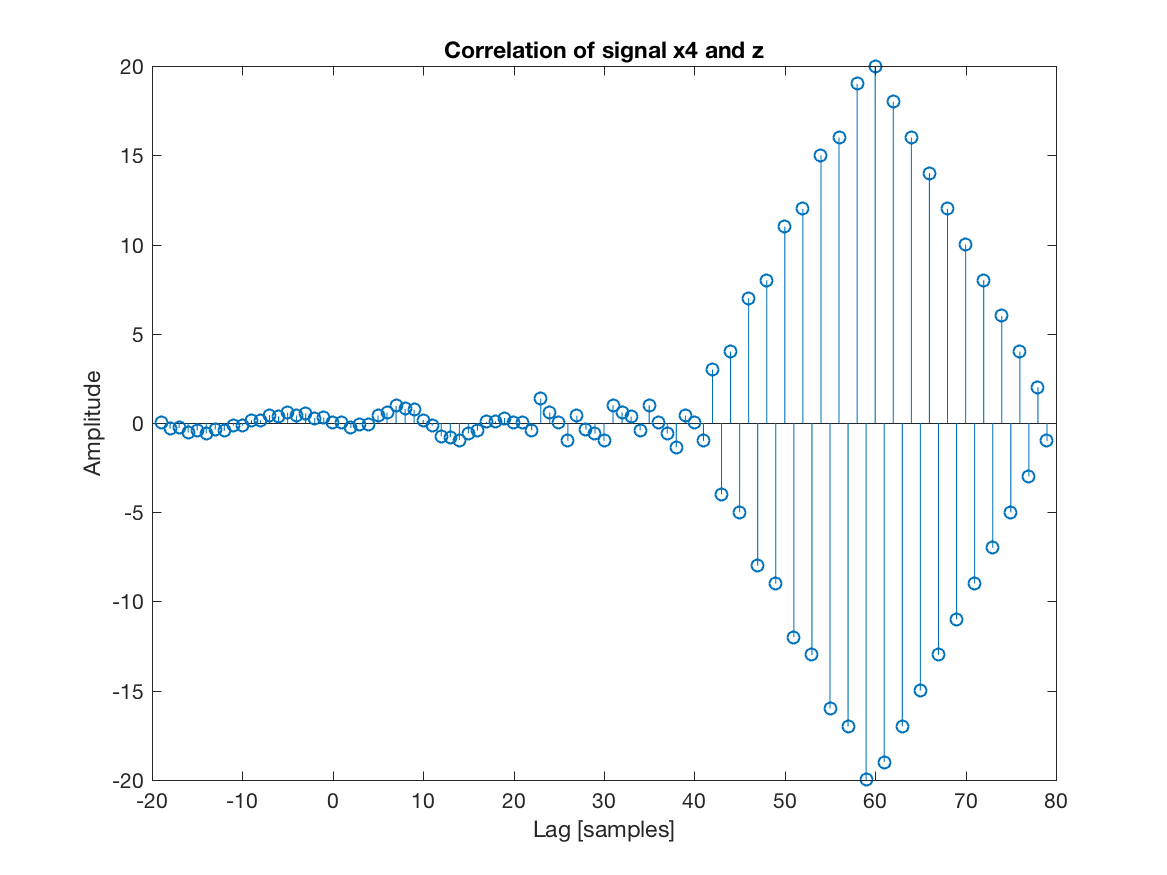
\includegraphics[width=1.7in,height=1.7in]{crossx4.png}
\caption{Correlations between signal z and signals x1, x2, x3, x4 respectively }
\label{fig:graph}
\end{figure}

\item It is clearly shown in the figure above that we can use the peak position of the correlation between the large signal $z[n]$ where the signals buried in and the single signal, i.e. where the correlation peaks, where the signal is the desired one. The index of the peak value is the ending index of signals buried in the large signal $z[n]$.

\end{enumerate}

\newpage
\Large\textbf{ Question \#5}:  \\
\normalsize My UFID is 21959681. The correlation os the code and message is shown below:\\
\begin{figure}[H]
\centering
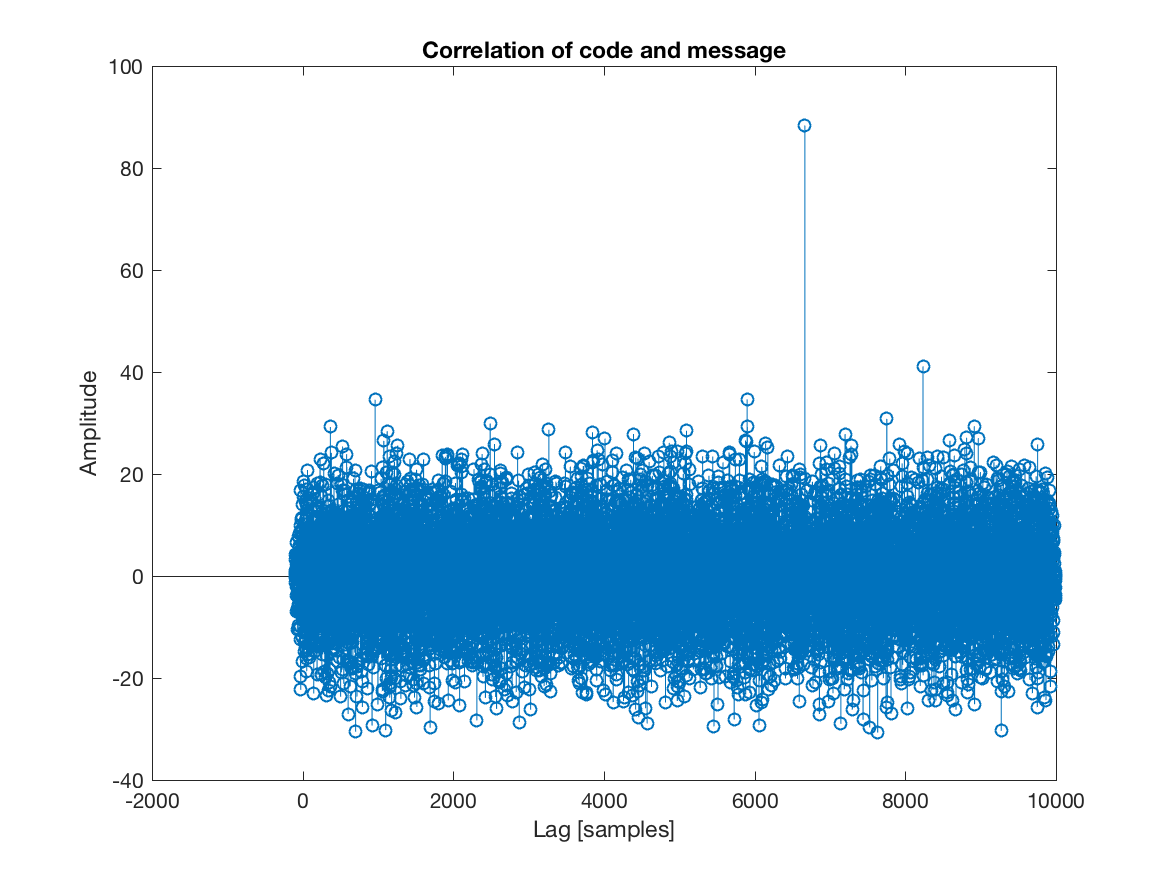
\includegraphics[width = 5in]{codemessage.png}
\caption{Correlation between code and message}
\end{figure}
The starting index with largest correlation is 6668.

\end{spacing}
\end{document}